\section{Experiments}
\label{sec:experiments}
We evaluate the effectiveness of the alignment learning framework by comparing its performance in terms of convergence speed, distance from human annotated ground truth durations, and speech quality. For autoregressive models like Flowtron and Tacotron 2, we compare with the baseline alignment methods therein. For FastPitch, we compare with an alignment method that relies on an external TTS model (Tacotron2) to obtain token durations. For the parallel models: FastSpeech 2 and RAD-TTS, we compare against an alignment method that obtains durations from the MFA aligner. We use the LJ Speech dataset (LJ)~\cite{LJS} for all our experiments. 

\subsection{Convergence Rate}
\begin{figure}[h]
    \begin{subfigure}{\linewidth}
    % \caption{Tacotron 2}
    \label{fig:taco2_mcd}
    % \vspace{-1\baselineskip}
    \hfill\begin{tikzpicture}[]
  \begin{axis}[
    height=3.0cm,
    width=0.9\linewidth,
      % xlabel= Iteration,
      % ylabel= {MCD-DTW},
      legend cell align={left},
      ylabel near ticks,
      xlabel near ticks,
      xlabel style= {font=\small},
      ylabel style={font=\small},
      legend style={font=\tiny},
      yticklabel style = {font=\tiny},
      xticklabel style = {font=\tiny},
      %ymode=log,
      xmin=600,
      xmax=24000,
      x tick label style={/pgf/number format/1000 sep=},  % sep={} disables comma in 1,000
      legend columns=1,
      legend entries={Tacotron 2, Tacotron 2 + prior, Tacotron 2 + prior + $\mathcal{L}_{\mathit{align}}$}
    ]
    \addplot [line width=0.3mm, color=lava] table [x=model, y=mel_cepstrum_mcd, y error=oursstd,col sep=comma] {\tacotronbasewopriormcd};
    \addplot [line width=0.3mm, color=glaucous] table [x=model, y=mel_cepstrum_mcd, y error=oursstd,col sep=comma] {\tacotronbaselinemcd};
    \addplot [line width=0.3mm, color=forestgreen] table [x=model, y=mel_cepstrum_mcd, y error=oursstd,col sep=comma] {\tacotronctcmcd};
  \end{axis}
\end{tikzpicture}\hspace{1.0cm}
 \end{subfigure}
 \begin{subfigure}[t]{\linewidth}
     % \caption{Flowtron Autoregressive}
     \label{fig:fta_mcd}
     % \vspace{-1\baselineskip}
     \hfill\begin{tikzpicture}[]
  \begin{axis}[
    height=3.2cm,
    width=0.9\linewidth,
      % xlabel= Iteration,
      % ylabel= {MCD-DTW},
      legend cell align={left},
      ylabel near ticks,
      % xlabel near ticks,
      xlabel style= {font=\small},
      ylabel style={font=\small},
      legend style={font=\tiny},
      yticklabel style = {font=\tiny},
      xticklabel style = {font=\tiny},
      x tick label style={
		/pgf/number format/1000 sep={}},
     % ymode=scale,
     % xmode=scale,
     xmin=0,
     xmax=48000,
      legend columns=1,
      legend entries={Flowtron (single-flow), Flowtron + prior, Flowtron + prior + $\mathcal{L}_{\mathit{align}}$ }
    ]
    \addplot [line width=0.3mm, color=lava] table [x=model, y=mel_cepstrum_mcd, y error=oursstd,col sep=comma] {\ftabasemcd};
    \addplot [line width=0.3mm, color=glaucous] table [x=model, y=mel_cepstrum_mcd, y error=oursstd,col sep=comma] {\ftabaselinemcd};
    \addplot [line width=0.3mm, color=forestgreen] table [x=model, y=mel_cepstrum_mcd, y error=oursstd,col sep=comma] {\ftactcmcd};
  \end{axis}
\end{tikzpicture}
\hspace{1.0cm}
 \end{subfigure}
 \begin{subfigure}[t]{\linewidth}
    % \caption{RAD-TTS}
    \label{fig:rad_tts_mcd}
    % \vspace{-1\baselineskip}
    \hfill\begin{tikzpicture}[]
  \begin{axis}[
    height=3.2cm,
    width=0.9\linewidth,
      % xlabel= Iteration,
      legend cell align={left},
      ylabel= {MCD-DTW},
      ylabel near ticks,
      xlabel near ticks,
      xlabel style= {font=\small},
      ylabel style={font=\small},
      legend style={font=\tiny},
      yticklabel style = {font=\tiny},
      xticklabel style = {font=\tiny},
      %ymode=log,
      xmin=500,
      xmax=19000,
      x tick label style={/pgf/number format/1000 sep=},  % sep={} disables comma in 1,000
      legend columns=1,
      legend entries={RadTTS (MFA durations), RadTTS w/o prior + $\mathcal{L}_{\mathit{align}}$, RadTTS with prior + $\mathcal{L}_{\mathit{align}}$}
    ]
    \addplot [line width=0.3mm, color=lava] table [x=iteration, y=mel_cepstrum_mcd, y error=oursstd,col sep=comma] {\ftpmfadtwsorted};
    
    
    \addplot [line width=0.3mm, color=glaucous] table [x=iteration, y=mel_cepstrum_mcd, y error=oursstd,col sep=comma] {\ftpnopriormcddtwsorted};
    
    \addplot [line width=0.3mm, color=forestgreen] table [x=iteration, y=mel_cepstrum_mcd, y error=oursstd,col sep=comma] {\ftpbetabinomialmcddtwsorted};
    
  \end{axis}
\end{tikzpicture}\hspace{1.0cm}
 \end{subfigure}
  \begin{subfigure}[t]{\linewidth}
    % \caption{FastPitch}
    \label{fig:fastpitch_mcd}
    % \vspace{-1\baselineskip}
     \hfill\begin{tikzpicture}[]
  \begin{axis}[
    height=3.2cm,
    width=0.9\linewidth,
      % xlabel= Iteration,
      ylabel= { },
      legend cell align={left},
      ylabel near ticks,
      xlabel near ticks,
      xlabel style= {font=\tiny},
      ylabel style={font=\tiny},
      legend style={font=\tiny},
      yticklabel style = {font=\tiny},
     xticklabel style = {font=\tiny},
      %ymode=log,
      xmin=500,
      xmax=5250,
      x tick label style={/pgf/number format/1000 sep=},  % sep={} disables comma in 1,000
      legend columns=1,
      legend entries={FastPitch (Tacotron 2 durations), FastPitch + prior + $\mathcal{L}_{\mathit{align}}$}
    ]
    \addplot [line width=0.3mm, color=lava] table [x=model, y=mel_cepstrum_mcd, y error=oursstd,col sep=comma] {\fastpitchbaselinemcd};
    \addplot [line width=0.3mm, color=forestgreen] table [x=model, y=mel_cepstrum_mcd, y error=oursstd,col sep=comma] {\fastpitchconvmcd};
  \end{axis}
\end{tikzpicture}
\hspace{1.0cm}
 \end{subfigure}
 \begin{subfigure}[t]{\linewidth}
    % \caption{FastSpeech2}
    \label{fig:fastspeech2_mcd}
    % \vspace{-1\baselineskip}
    \hfill\begin{tikzpicture}[]
  \begin{axis}[
    height=3.2cm,
    width=0.9\linewidth,
      xlabel= Iteration,
      % ylabel= {MCD-DTW},
      legend cell align={left},
      ylabel near ticks,
      xlabel near ticks,
      xlabel style= {font=\small},
      ylabel style={font=\tiny},
      legend style={font=\tiny},
      yticklabel style = {font=\tiny},
      xticklabel style = {font=\tiny},
      %ymode=log,
      xmin=4000,
      xmax=98000,
      x tick label style={/pgf/number format/1000 sep=},  % sep={} disables comma in 1,000
      legend columns=1,
      legend entries={FastSpeech 2 (MFA durations), FastSpeech 2 + prior + $\mathcal{L}_{\mathit{align}}$}
    ]
    \addplot [line width=0.3mm, color=lava] table [x=model, y=mel_cepstrum_mcd, y error=oursstd,col sep=comma] {\fastspeechbaseline};
    \addplot [line width=0.3mm, color=forestgreen] table [x=model, y=mel_cepstrum_mcd, y error=oursstd,col sep=comma] {\fastspeechconvattn};
  \end{axis}
\end{tikzpicture}
\hspace{1.0cm}
 \end{subfigure}
 \caption{Convergence rate improvements in TTS models with the alignment learning framework}
 % as an approximate L2 error on synthesized samples from early checkpoints. Fig. \ref{fig:duration_difference} looks at the mean alignment error measured against 10 annotated phrases.}
 \label{fig:mcd}
 \vspace*{-1\baselineskip}
\end{figure}

In order to compare the convergence rate of different alignment methods, we use the mean mel-cepstral distance (MCD)~\cite{mcd, Battenberg}. MCD compares the distance between synthesized and ground truth mel-spectrograms aligned temporarily with dynamic time warping (DTW). We observe in Figure~\ref{fig:mcd} that using the static prior described in Section~\ref{sec:accelerating_alignments} significantly improves the convergence rate of Tacotron2. Parallel models such as RAD-TTS, FastPitch, and FastSpeech2 with the alignment framework (no dependency on external aligners) converge at the same rate as their baseline models using a forced aligner. The model that benefits the most from using the alignment framework is Flowtron. It has two autoregressive flows running in opposing directions, each with their own learned alignment. Notably, the second autoregressive flow is performed on top of the autoregressive outputs of the previous flow. This means that if the alignment in the first flow fails, so will the second. Training is very slow as the second flow can only be added after the first has converged. Prior attempts to train both flows simultaneously have resulted in poor minima where neither flow has learned to align. By using just the attention prior, we are now able to train at least two flows simultaneously, with further improvements with adding the unsupervised alignment learning $\mathcal{L}_{\mathit{align}}$ objective described in Section~\ref{sec:ctc_objective}. This significantly reduces training time and improves convergence of Flowtron. 

%The baseline model shown in the figure has a single flow, while the ones with the prior and $\mathcal{L}_{\mathit{align}}$ have two steps of flow, what makes the difference even more striking.

%has multiple steps of flows, with every other flow operating in the opposite direction, learning the alignments without the prior is more challenging and we were unable to converge to reasonable alignment without the prior when attempting to learn 2 steps of flow simultaneously. Hence, we attempt to learn a single step of flow application of the prior significantly enhances convergence. We observe a similar boost in convergence speed in non autoregressive models like RAD-TTS as demonstrated in Figure~ \ref{fig:rad_tts_mcd}. 
\begin{figure*}
 \begin{subfigure}{0.25\textwidth}
    \centering
    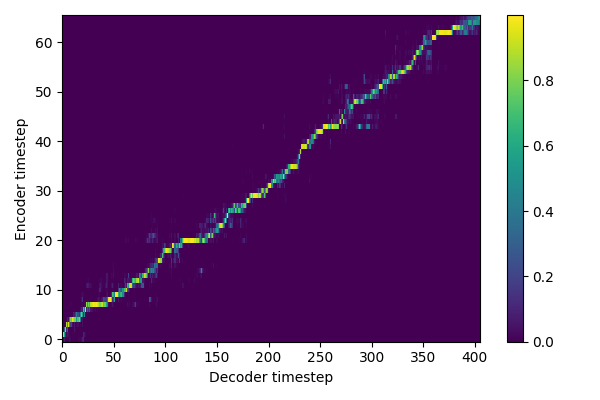
\includegraphics[width=\linewidth]{images/fta_baseline.png}
    \caption{Flowtron}
    \label{fig:fta_base_align}
\end{subfigure}
\begin{subfigure}{0.25\textwidth}
\centering
  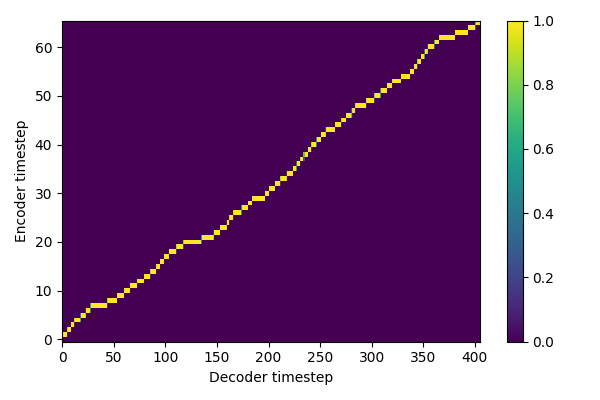
\includegraphics[width=\linewidth]{images/fta_with_alignment.png}
  \caption{Flowtron with $\mathcal{L}_{\mathit{align}}$}
  \label{fig:fta_ctc_align}
\end{subfigure}
 \begin{subfigure}{0.25\textwidth}
 \centering
  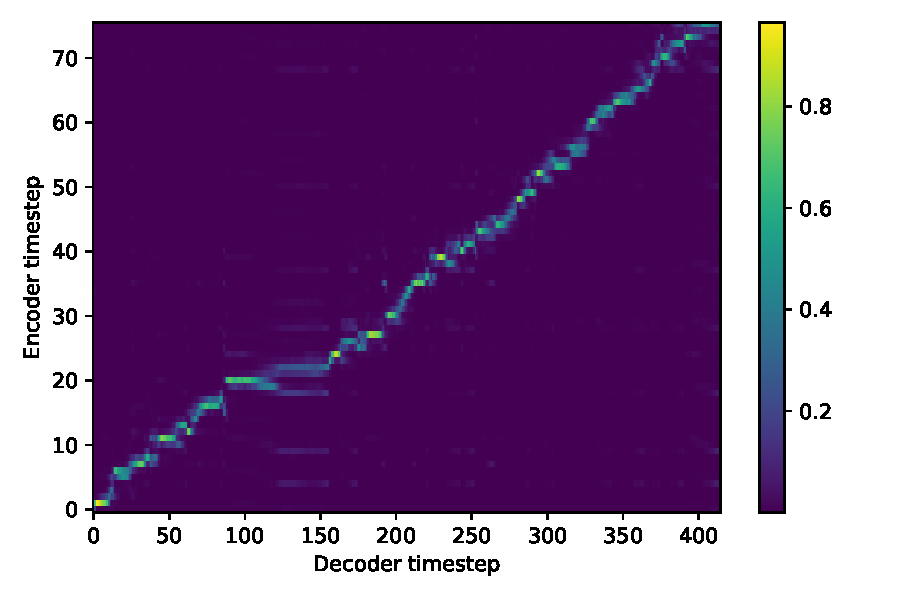
\includegraphics[width=\linewidth]{images/taco2_base.pdf}
  \caption{Tacotron 2}
  \label{fig:taco2_base_align}
\end{subfigure}%
\begin{subfigure}{0.25\textwidth}
\centering
  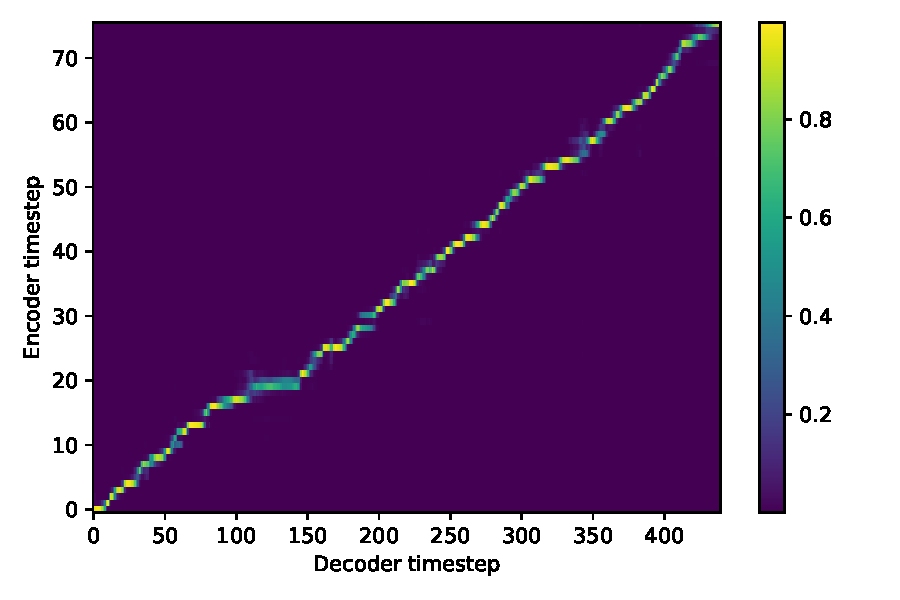
\includegraphics[width=\linewidth]{images/taco2_ctc.pdf}
  \caption{Tacotron 2 with $\mathcal{L}_{\mathit{align}}$}
  \label{fig:taco2_ctc_align}
\end{subfigure}
\caption{Converged soft alignments for Flowtron, Tacotron2. Alignment framework provides sharper and more connected alignments.}
\label{fig:align_convergence}
\vspace*{-1.5\baselineskip}
\end{figure*}

\subsection{Alignment Sharpness}
We visually inspect alignment matrices for a specific validation sample in Figure~\ref{fig:align_convergence}. The alignment objective consistently makes the attention distribution sharper with more connected alignment paths. This suggests that models with $\mathcal{L}_{\mathit{align}}$ produce more confident and continuous alignments, and by extension, continuous speech without repeating or missing words. 

\begin{figure}[h]
% \begin{subfigure}{\linewidth}
%     \caption{Flowtron Duration Distance}
%     \label{fig:flowtron_duration_diff}
%     \vspace{\baselineskip}
%     \begin{center}
\begin{tikzpicture}[scale=1.0]
  \begin{axis}[
  height=6.0cm,
  width=0.9\linewidth,
      xlabel= Iteration,
      ylabel= {Alignment error},
      ylabel near ticks,
      xlabel near ticks,
      xlabel style={font=\small},
      ylabel style={font=\small},
      yticklabel style = {font=\tiny},
      xticklabel style = {font=\tiny},
      legend style={font=\tiny},
      legend columns=1,
      legend entries={Flowtron, Flowtron CTC guided, tactron baseline, tacotron CTC guided}
    ]
    \addplot [line width=0.3mm, color=lava] table [x=iteration, y=phoneme_l1_distance, y error=oursstd,col sep=comma] {\ftabasedurationdistance};
    \addplot [line width=0.3mm, color=forestgreen] table [x=iteration, y=phoneme_l1_distance, y error=oursstd,col sep=comma] {\ftactcdurationdistance};
    \addplot [line width=0.3mm, color=glaucous] table [x=iteration, y=phoneme_l1_distance, y error=oursstd,col sep=comma] {\tacotronbasedurationdistance};
    \addplot [line width=0.3mm, color=] table [x=iteration, y=phoneme_l1_distance, y error=oursstd,col sep=comma] {\tacotronctcdurationdistance};
  \end{axis}
\end{tikzpicture}
\end{center}

%  \end{subfigure}
\begin{subfigure}{\linewidth}
    % \caption{Flowtron Duration Distance}
    \label{fig:flowtron_duration_diff}
    %\vspace{-1\baselineskip}
    \hfill\begin{tikzpicture}[scale=1.0]
  \begin{axis}[
  height=3.0cm,
  width=0.9\linewidth,
      % xlabel= Iteration,
      % ylabel= {Alignment error},
      legend cell align={left},
      ylabel near ticks,
      xlabel near ticks,
      xlabel style={font=\small},
      ylabel style={font=\small},
      yticklabel style = {font=\tiny},
      xticklabel style = {font=\tiny},
      x tick label style={/pgf/number format/1000 sep=},  % sep={} disables comma in 1,000
      xmin=0,
      xmax=230000,
      legend style={font=\tiny},
      legend columns=1,
      legend entries={Flowtron, Flowtron + prior + $\mathcal{L}_{\mathit{align}}$}
    ]
    \addplot [line width=0.3mm, color=lava] table [x=iteration, y=phoneme_l1_distance, y error=oursstd,col sep=comma] {\ftabasedurationdistance};
    \addplot [line width=0.3mm, color=forestgreen] table [x=iteration, y=phoneme_l1_distance, y error=oursstd,col sep=comma] {\ftactcdurationdistance};
    
  \end{axis}
\end{tikzpicture}\hspace{1.0cm}
 \end{subfigure}
 \begin{subfigure}{\linewidth}
    % \caption{Tacotron 2 Duration Distance}
    \label{fig:tacotron_duration_diff}
    \vspace{-1.2cm}  %\baselineskip}
    \hfill\begin{tikzpicture}[scale=1.0]
  \begin{axis}[
  height=3.0cm,
  width=0.9\linewidth,
      legend cell align={left},
      xlabel= Iteration,
      ylabel= {Alignment error},
      ylabel near ticks,
      y label style={at={(-0.07,1.2)}},
      xlabel near ticks,
      xlabel style={font=\small},
      ylabel style={font=\small},
      yticklabel style = {font=\tiny},
      xticklabel style = {font=\tiny},
      x tick label style={/pgf/number format/1000 sep=},  % sep={} disables comma in 1,000
      xmin=0,
      xmax=29000,
      legend style={font=\tiny},
      legend columns=1,
      legend entries={Tacotron 2, Tacotron 2 + prior + $\mathcal{L}_{\mathit{align}}$}
    ]
    \addplot [line width=0.3mm, color=lava] table [x=iteration, y=phoneme_l1_distance, y error=oursstd,col sep=comma] {\tacotronbasedurationdistance};
    \addplot [line width=0.3mm, color=forestgreen] table [x=iteration, y=phoneme_l1_distance, y error=oursstd,col sep=comma] {\tacotronctcdurationdistance};
    
  \end{axis}
\end{tikzpicture}
\hspace{1.0cm}
 \end{subfigure}
 \vspace{-1\baselineskip}
 \caption{$L_1$ distance between ground truth alignments and those extracted during training for Flowtron and Tacotron 2. Both use different batch sizes and are thus plotted separately. % (Fig \ref{fig:flowtron_duration_diff}),
 % (Fig \ref{fig:tacotron_duration_diff}) 
 }
 \label{fig:duration_diff}
 \vspace*{-1.5\baselineskip}
\end{figure}

\subsection{Duration Analysis}
In order to observe the influence of the unsupervised alignment loss on the quality of alignments, we compare phoneme durations extracted from model alignments to manually annotated phoneme durations from 10 samples of the LJ test set. For autoregressive models, we extract the binarized alignments from soft alignments using a monotonic argmax, iterating through phonemes and identifying the phoneme with maximum attention weights among the current and next phonemes. We use this binarized alignment to extract durations for each phoneme. Figure~\ref{fig:duration_diff} shows the average $L_1$ distance between durations extracted from the models with respect to ground truth annotated durations. By using our alignment framework we obtain a faster convergence rate than the baseline and alignments closer to the ground truth.

% \begin{figure*}[t]
%  \begin{subfigure}[t]{0.25\textwidth}
%     \centering
%     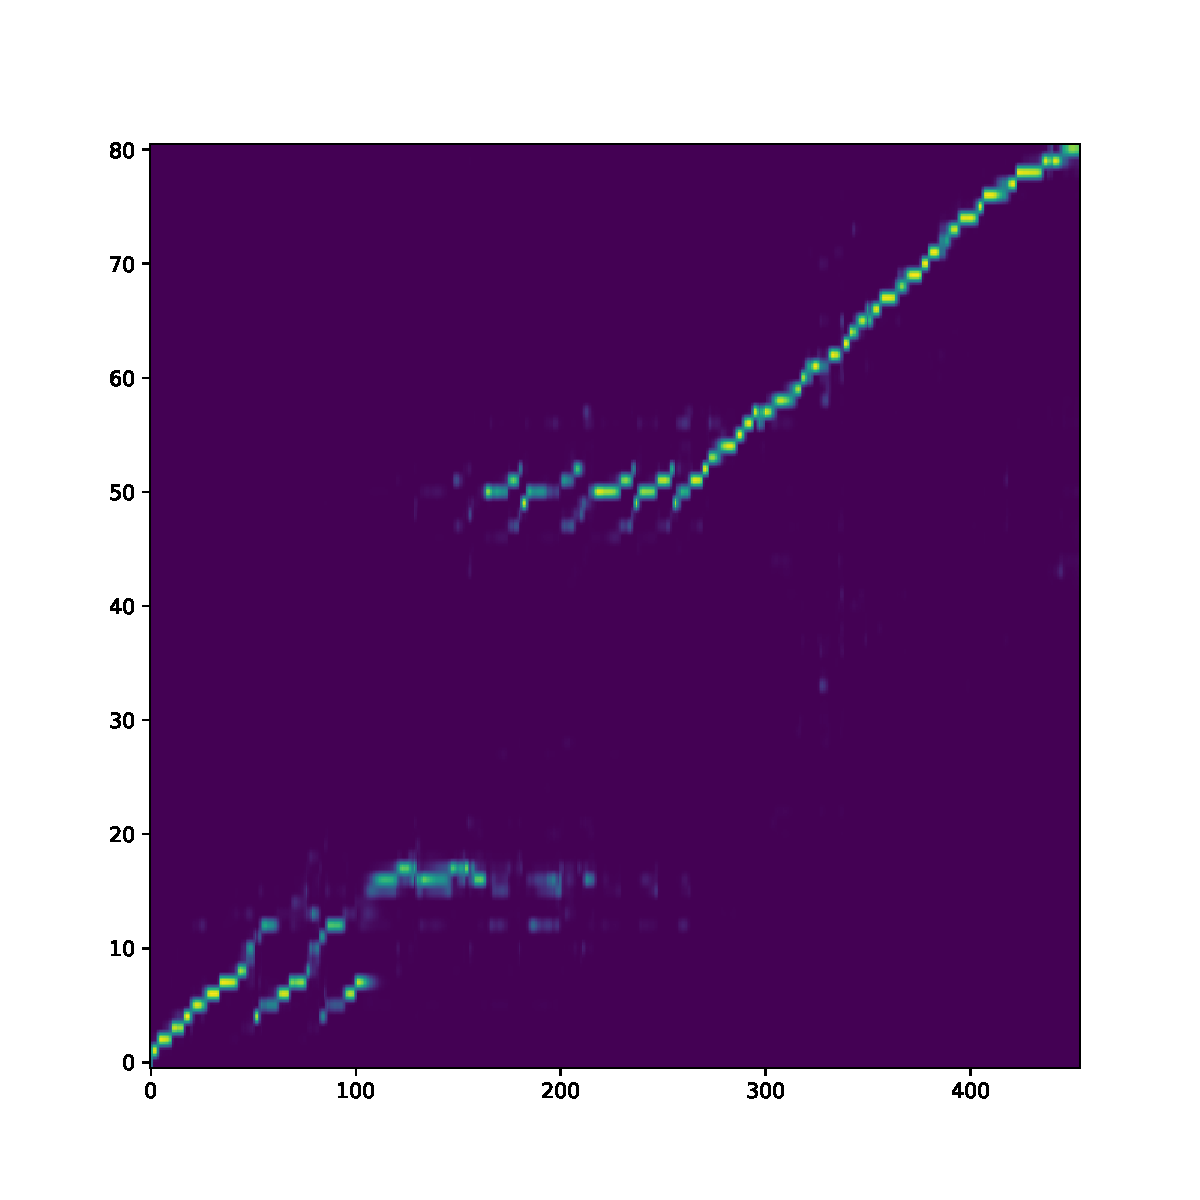
\includegraphics[width=\linewidth]{images/convergence_flowtron_base_soft.pdf}
%     \caption{Flowtron Baseline soft alignments}
%     \label{fig:conv_fta_base_soft}
% \end{subfigure}
% \begin{subfigure}[t]{0.25\textwidth}
% \centering
%   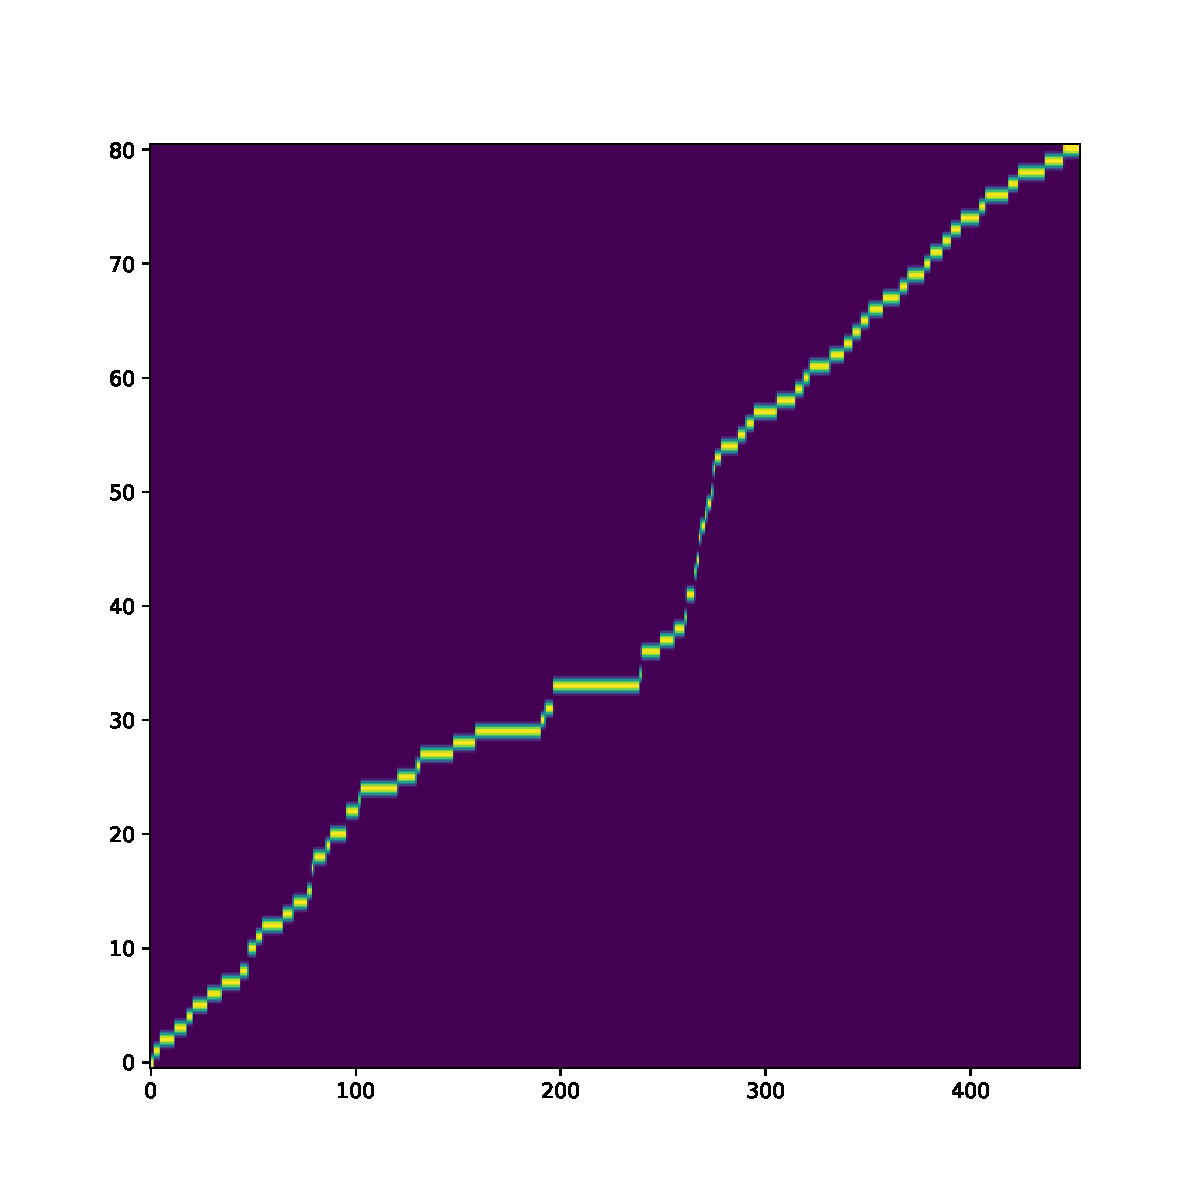
\includegraphics[width=\linewidth]{images/convergence_flowtron_base_margmax.pdf}
%   \caption{Flowtron Baseline monotonic argmax alignment}
%   \label{fig:6k_with_prior}
% \end{subfigure}
%  \begin{subfigure}[t]{0.25\textwidth}
%  \centering
%   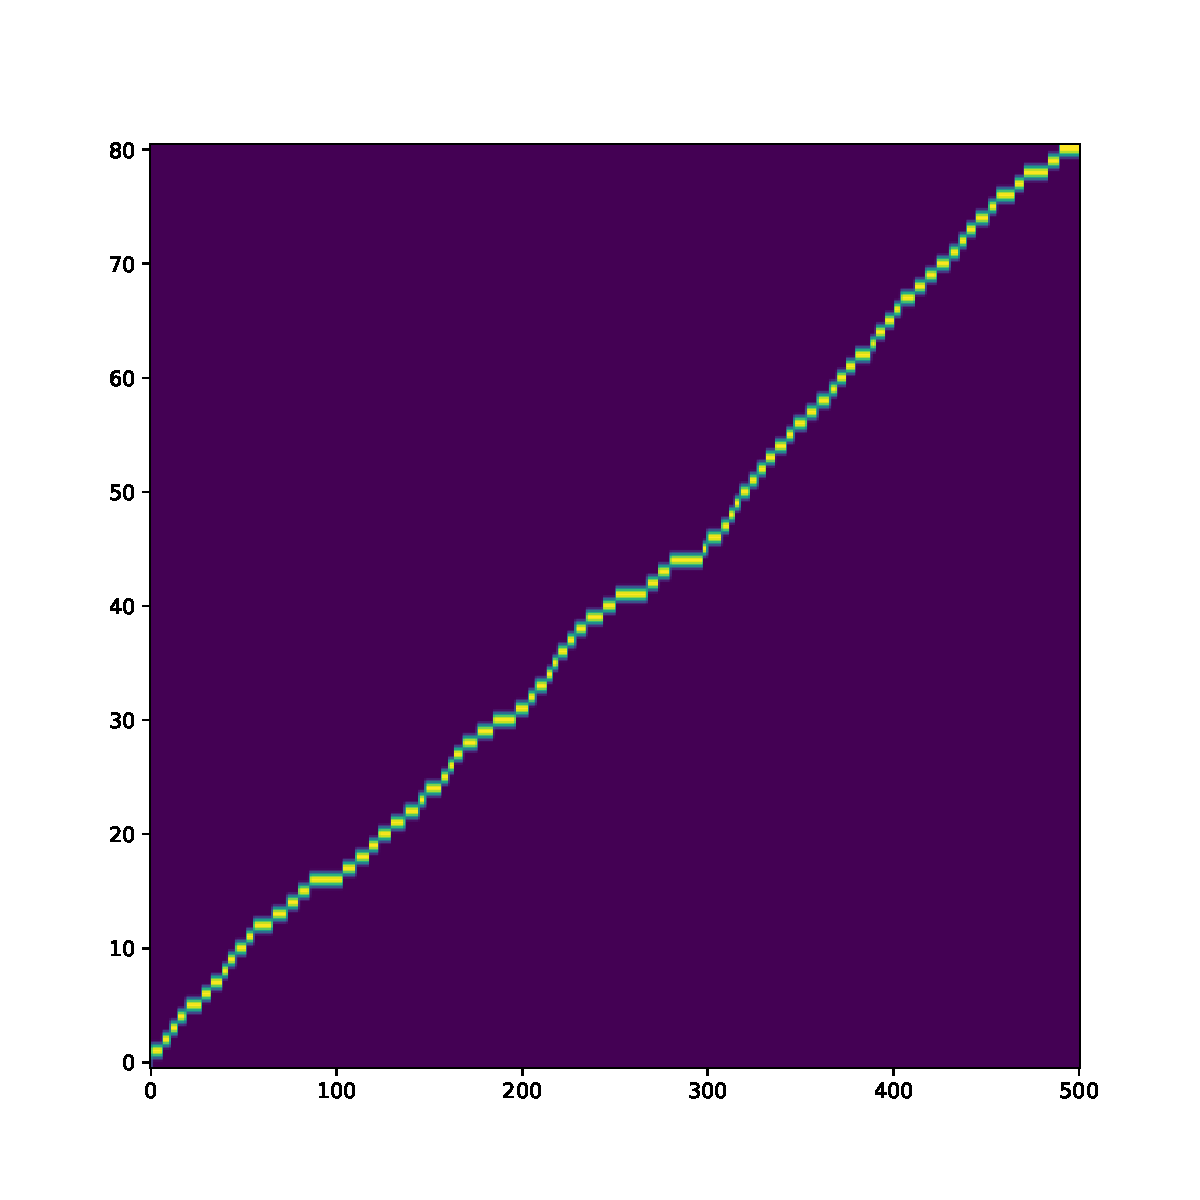
\includegraphics[width=\linewidth]{images/convergence_flowtron_ctc_soft.pdf}
%   \caption{Flowtron CTC guided monotonic soft alignment}
%   \label{fig:108k_without_prior}
% \end{subfigure}%
% \begin{subfigure}[t]{0.25\textwidth}
% \centering
%   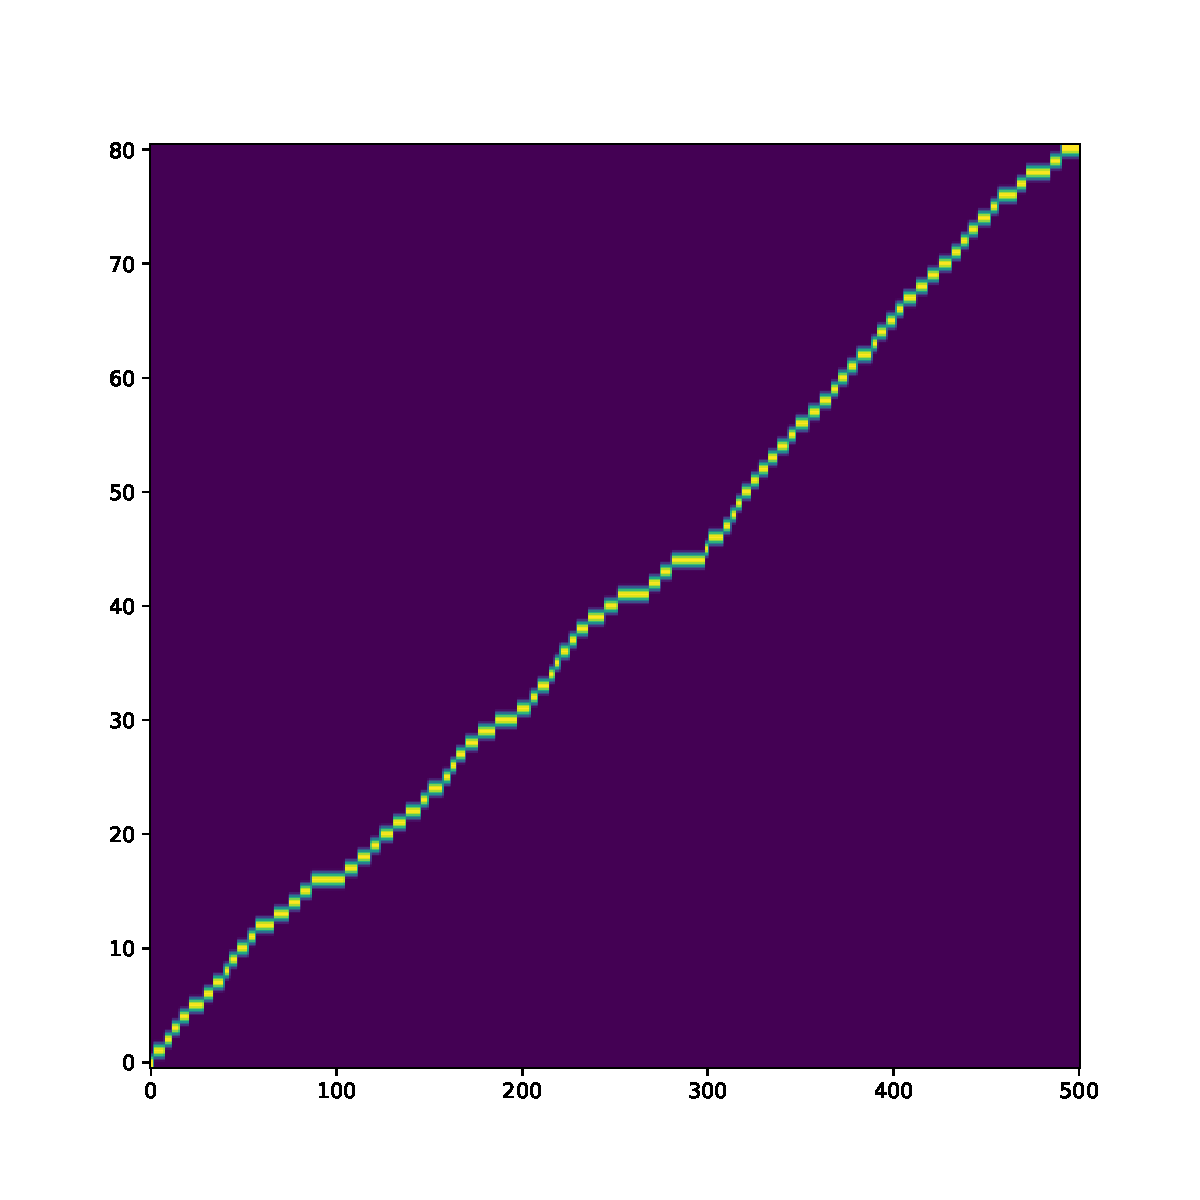
\includegraphics[width=\linewidth]{images/convergence_flowtron_ctc_margmax.pdf}
%   \caption{Flowtron CTC guided monotonic argmax alignment}
%   \label{fig:108k_with_prior}
% \end{subfigure}
% \caption{Inference alignment maps extracted from Flowtron baseline [add ref] and CTC guided flowtron [add fig ref]}
% \label{fig:align_speedup}
% \end{figure*}


\subsection{Pairwise Opinion Scores}
%A side by side pairwise evaluation was conducted over 100 LJ test set samples from the  where participants were shown samples from 2 models on either side and were asked to select the better sample. We crowd-sourced pairwise preference tests on Amazon Mechanical Turk. The raters were asked to count sinusoids as part of a hearing test in order to be eligible for rating.
We crowd-sourced pairwise preference scores to subjectively compare models trained with our alignment learning framework against baseline. Listeners were pre-screened with a hearing test based on sinusoid counting. During the pairwise ranking, raters were repeatedly given two synthesized utterances of the same text, picked at random from 100 LJ test samples. Both were synthesized with the same architecture: one being the baseline, and other using our alignment framework. The listeners were shown the text and asked to select samples with the best overall quality, defined by accuracy of text, its pleasantness and naturalness. Approximately 200 scores per model were collected. Table~\ref{tab:pairwise_results} shows pairwise preference scores of models trained with alignment framework over baseline. It shows that the alignment framework consistently improves over all baselines.

\begin{table}[!ht]
    %\tiny
    \caption{Pairwise preference scores judged by human raters, shown with $95\%$ confidence intervals. Scores above 0.5 indicate models trained with $\mathcal{L}_{\mathit{align}}$ were preferred by majority of raters.}
    \centering
    \begin{tabular}{lc}
        \toprule
        \textbf{Model} & \textbf{ Alignment Framework vs Baseline}\\
        \midrule
        Tacotron 2  & $0.556 \pm 0.068$ \\
        Flowtron $(\sigma = .5)$ & $0.635 \pm 0.065$ \\
        RAD-TTS $(\sigma = .5)$ & $0.639 \pm 0.066$ \\
        FastPitch & $0.565 \pm 0.068$ \\
        FastSpeech2 & $0.521 \pm 0.067$ \\
        \bottomrule
        \end{tabular}
    \vspace{-1.5\baselineskip}
    \label{tab:pairwise_results}
    
\end{table}
\subsection{Robustness to Errors on Long Utterances}
We measure character error rate (CER) between synthesized and input texts using an external speech recognition model to evaluate the robustness of the alignments on long utterances. We use $14,045$ full sentences from the LibriTTS dataset~\cite{libritts}. We synthesize speech with models trained on LJ Speech, and recognize it with Jasper~\cite{li2019jasper}. Figure~\ref{fig:cer} shows that autoregressive models with $\mathcal{L}_{\mathit{align}}$ have a lower CER, providing evidence that the alignment objective results in more robust speech for long utterances. Parallel models such as RAD-TTS use a duration predictor and do not suffer from alignment issues, and hence have a much lower CER than autoregressive models. 

%, selected for the least punctuation and no proper nouns.

\begin{figure}[h]
% \begin{subfigure}{\linewidth}
%     \caption{Flowtron Duration Distance}
%     \label{fig:flowtron_duration_diff}
%     \vspace{\baselineskip}
%     \begin{center}
\begin{tikzpicture}[scale=1.0]
  \begin{axis}[
  height=6.0cm,
  width=0.9\linewidth,
      xlabel= Iteration,
      ylabel= {Alignment error},
      ylabel near ticks,
      xlabel near ticks,
      xlabel style={font=\small},
      ylabel style={font=\small},
      yticklabel style = {font=\tiny},
      xticklabel style = {font=\tiny},
      legend style={font=\tiny},
      legend columns=1,
      legend entries={Flowtron, Flowtron CTC guided, tactron baseline, tacotron CTC guided}
    ]
    \addplot [line width=0.3mm, color=lava] table [x=iteration, y=phoneme_l1_distance, y error=oursstd,col sep=comma] {\ftabasedurationdistance};
    \addplot [line width=0.3mm, color=forestgreen] table [x=iteration, y=phoneme_l1_distance, y error=oursstd,col sep=comma] {\ftactcdurationdistance};
    \addplot [line width=0.3mm, color=glaucous] table [x=iteration, y=phoneme_l1_distance, y error=oursstd,col sep=comma] {\tacotronbasedurationdistance};
    \addplot [line width=0.3mm, color=] table [x=iteration, y=phoneme_l1_distance, y error=oursstd,col sep=comma] {\tacotronctcdurationdistance};
  \end{axis}
\end{tikzpicture}
\end{center}

    
%  \end{subfigure}
% \begin{subfigure}{\linewidth}
%     %\label{fig:flowtron_cer}
%     %\vspace{-1\baselineskip}
%     \begin{center}
\begin{tikzpicture}[scale=1.0]
  \begin{axis}[
  height=3.5cm,
  width=0.98\linewidth,
      %xlabel= {Character Length},
      legend cell align={left},
      ylabel= {CER},
      ylabel near ticks,
      xlabel near ticks,
      xlabel style={font=\small},
      ylabel style={font=\small},
      yticklabel style = {font=\tiny},
      xticklabel style = {font=\tiny},
      xmin=40,
      xmax=400,
      x tick label style={/pgf/number format/1000 sep=},  % sep={} disables comma in 1,000
      legend style={font=\tiny},
      legend columns=1,
      legend style={at={(0,1)},anchor=north west},
      legend entries={Flowtron, Flowtron + prior + $\mathcal{L}_{\mathit{align}}$} 
    ]
    \addplot [line width=0.3mm, color=lava] table [x=text_len, y=mean_cer, y error=oursstd,col sep=comma] {\ftacerbase};
    \addplot [line width=0.3mm, color=forestgreen] table [x=text_len, y=mean_cer, y error=oursstd,col sep=comma] {\ftacerctc};
    % \addplot [line width=0.3mm, color=brightube] table [x=text_len, y=mean_cer, y error=oursstd,col sep=comma] {\tacocerbase};
    % \addplot [line width=0.3mm, color=fulvous] table [x=text_len, y=mean_cer, y error=oursstd,col sep=comma] {\tacocerctc};
    % \addplot [line width=0.3mm, color=glaucous] table [x=text_len, y=mean_cer, y error=oursstd,col sep=comma] {\ftpcer};
  \end{axis}
\end{tikzpicture}
\end{center}

%  \end{subfigure}
 \begin{subfigure}{\linewidth}
    %\label{fig:tacotron_cer}
    \begin{center}
\begin{tikzpicture}[scale=1.0]
  \begin{axis}[
  height=3.5cm,
  width=0.98\linewidth,
      legend cell align={left},
      xlabel= {Text Length},
      ylabel= {CER},
      ylabel near ticks,
      xlabel near ticks,
      xlabel style={font=\small},
      ylabel style={font=\small},
      yticklabel style = {font=\tiny},
      xticklabel style = {font=\tiny},
      xmin=40,
      xmax=1200,
      x tick label style={/pgf/number format/1000 sep=},  % sep={} disables comma in 1,000
      legend style={font=\tiny},
      legend style={at={(-0.1,-0.5)},anchor=north west},
      legend columns=3,
      legend entries={Tacotron2, Tacotron2 + prior + $\mathcal{L}_{\mathit{align}}$, Rad-TTS + prior + $\mathcal{L}_{\mathit{align}}$, Flowtron, Flowtron + prior + $\mathcal{L}_{\mathit{align}}$}
    ]
    \addplot [dashed, line width=0.3mm, color=brightube] table [x=text_len, y=mean_cer, y error=oursstd,col sep=comma] {\tacocerbase};
    \addplot [line width=0.3mm, color=fulvous] table [x=text_len, y=mean_cer, y error=oursstd,col sep=comma] {\tacocerctc};
    \addplot [line width=0.3mm, color=glaucous] table [x=text_len, y=mean_cer, y error=oursstd,col sep=comma] {\ftpcer};
    \addplot [dashed, line width=0.3mm, color=lava] table [x=text_len, y=mean_cer, y error=oursstd,col sep=comma] {\ftacerbase};
    \addplot [line width=0.3mm, color=forestgreen] table [x=text_len, y=mean_cer, y error=oursstd,col sep=comma] {\ftacerctc};
    
  \end{axis}
\end{tikzpicture}
\end{center}

    \vspace{-1.0\baselineskip}
 \end{subfigure}
%  \begin{subfigure}{\linewidth}
%     \caption{Tacotron 2 Duration Distance}
%     \label{fig:tacotron_duration_diff}
%     \vspace{-2\baselineskip}
%     \begin{tikzpicture}[scale=1.0]
  \begin{axis}[
  height=3.0cm,
  width=0.9\linewidth,
      legend cell align={left},
      xlabel= Iteration,
      ylabel= {Alignment error},
      ylabel near ticks,
      y label style={at={(-0.07,1.2)}},
      xlabel near ticks,
      xlabel style={font=\small},
      ylabel style={font=\small},
      yticklabel style = {font=\tiny},
      xticklabel style = {font=\tiny},
      x tick label style={/pgf/number format/1000 sep=},  % sep={} disables comma in 1,000
      xmin=0,
      xmax=29000,
      legend style={font=\tiny},
      legend columns=1,
      legend entries={Tacotron 2, Tacotron 2 + prior + $\mathcal{L}_{\mathit{align}}$}
    ]
    \addplot [line width=0.3mm, color=lava] table [x=iteration, y=phoneme_l1_distance, y error=oursstd,col sep=comma] {\tacotronbasedurationdistance};
    \addplot [line width=0.3mm, color=forestgreen] table [x=iteration, y=phoneme_l1_distance, y error=oursstd,col sep=comma] {\tacotronctcdurationdistance};
    
  \end{axis}
\end{tikzpicture}

%  \end{subfigure}
 \caption{Character error rate of different models at different text lengths. Models that use the alignment framework make fewer mistakes with increased utterance length.}
%  The $\mathcal{L}_{\mathit{align}}$ results in lower CER than baseline.}
 \label{fig:cer}
 \vspace*{-1.5\baselineskip}
\end{figure}